\documentclass{article}%
\usepackage[T1]{fontenc}%
\usepackage[utf8]{inputenc}%
\usepackage{lmodern}%
\usepackage{textcomp}%
\usepackage{lastpage}%
\usepackage{geometry}%
\geometry{margin=1in}%
\usepackage{graphicx}%
%
\usepackage{amsmath}%
\usepackage{amssymb}%
\usepackage{booktabs}%
\usepackage{longtable}%
\usepackage{float}%
\usepackage{caption}%
\usepackage{hyperref}%
\title{CHE 565 {-}{-} Homework 4}%
\author{Soki Sem}%
\date{\today}%
%
\begin{document}%
\normalsize%
\setlength{\parindent}{0pt}%
\setlength{\parskip}{0.6em}%
\maketitle%
\section*{Untitled Section}%
\label{sec:UntitledSection}%
\subsection*{Controller Design using  $\lambda$  -Rules}%
\label{subsec:ControllerDesignusinglambda{-}Rules}%
\[%
\lambda = \max\left(\frac{\tau_p}{3}, \theta \right)%
\]%
\begin{align*}%
\lambda &= \max\left(\frac{5}{3}, 1\right) \\%
&= \frac{5}{3} \approx 1.667%
\end{align*}%
\[%
K_c = \frac{\tau_p}{K_p(\lambda + \theta)}%
\]%
\begin{align*}%
K_c &= \frac{5}{1(1.667 + 1)} \\%
&= \frac{5}{2.667} \\%
&\approx 1.875%
\end{align*}%
\[%
\tau_I = \tau_p%
\]%
\begin{align*}%
\tau_I &= 5%
\end{align*}%
\[%
I = \frac{1}{\tau_I}%
\]%
\begin{align*}%
I &= \frac{1}{5} \\%
&= 0.2%
\end{align*}

%
\subsection*{Controller Transfer Function}%
\label{subsec:ControllerTransferFunction}%
\[%
G_c(s) = K_c \left(1 + \frac{1}{\tau_I s} \right)%
\]%
\begin{align*}%
G_c(s) &= 1.875 \left(1 + \frac{1}{5s} \right) \\%
&= 1.875 + \frac{0.375}{s}%
\end{align*}

%
\subsection*{Closed{-}Loop System}%
\label{subsec:Closed{-}LoopSystem}%
The control system is arranged in a standard feedback configuration.%
\par%
\[%
E = Y_{sp} - Y%
\]%
\[%
Y_c = G_c(s)E%
\]%
The disturbance is added after the controller output.%
\par%
\[%
P = Y_c + d%
\]%
\[%
Y = G_p(s) P%
\]

%
\subsection*{Simulation Cases}%
\label{subsec:SimulationCases}%
The following simulations were performed:%
\par%
1. Step change in setpoint (magnitude 1), no disturbance%
\par%
2. Step change in disturbance (magnitude 1), no setpoint change%
\par%
3. Double controller gain%
\par%
4. Half controller gain%
\par%
5. Increased and decreased integral time constant%
\par

%
\subsection*{Disturbance Response}%
\label{subsec:DisturbanceResponse}%
A unit step disturbance was applied with no setpoint change.%
\par%
\[%
Y_{sp}(t) = 0, \quad d(t) = 1%
\]

%
\subsection*{Effect of Controller Gain}%
\label{subsec:EffectofControllerGain}%
The controller gain was varied to observe its effect on system response.%
\par%
\[%
K_c = 2K_c^{\text{nominal}}%
\]%
\[%
K_c = 0.5K_c^{\text{nominal}}%
\]

%
\subsection*{Effect of Integral Time Constant}%
\label{subsec:EffectofIntegralTimeConstant}%

%
\section*{Problem 1}%
\label{sec:Problem1}%
A closed{-}loop control system was constructed for the process%
\par%
\[%
G_p(s)=\frac{e^{-s}}{5s+1}%
\]%
with a disturbance added after the controller. The controller was set to ideal PI form, as required in the assignment.%
\par%
\subsection*{1. Controller Settings from the $\lambda$-Rules}%
\label{subsec:1.ControllerSettingsfromthelambda{-}Rules}%
For the given process model, the process gain, time constant, and dead time are identified as%
\par%
\[%
K_p=1,\qquad \tau_p=5,\qquad \theta=1%
\]%
The assignment specifies that%
\par%
\[%
\lambda=\max\left(\frac{\tau_p}{3},\theta\right)%
\]%
\begin{align*}%
\lambda &= \max\left(\frac{5}{3},1\right) \\%
&= \frac{5}{3}\approx 1.667%
\end{align*}%
For PI control using the lambda tuning rules for a first{-}order plus dead{-}time model,%
\par%
\[%
K_c=\frac{\tau_p}{K_p(\lambda+\theta)}, \qquad \tau_I=\tau_p%
\]%
\begin{align*}%
K_c &= \frac{5}{1(1.667+1)} \\%
&= \frac{5}{2.667} \\%
&= 1.8750%
\end{align*}%
\begin{align*}%
\tau_I &= 5.0000%
\end{align*}%
Because Simulink uses the reset rate instead of the integral time constant,%
\par%
\[%
I=\frac{1}{\tau_I}%
\]%
\begin{align*}%
I &= \frac{1}{5.0000} \\%
&= 0.2000%
\end{align*}%
Therefore, the controller settings entered into Simulink were%
\par%
\begin{align*}%
P &= K_c = 1.8750 \\%
I &= 0.2000%
\end{align*}

%
\subsection*{2. Step Change in Setpoint, No Disturbance}%
\label{subsec:2.StepChangeinSetpoint,NoDisturbance}%
A unit step was applied to the setpoint while the disturbance was held at zero.%
\par%
\[%
Y_{{sp}}(t)=1,\qquad d(t)=0%
\]%


\begin{figure}[H]%
\centering%

\includegraphics[width=0.95\textwidth]{part2_setpoint_nominal.png}%
\caption{Closed{-}loop response for a unit step change in setpoint with no disturbance, using the nominal PI settings.}%
\label{fig:fig1}%
\end{figure}

%
\[%
\text{The response of the closed-loop system is shown in Figure} \ref{fig:fig1} \text{for the nominal PI settings obtained from the $\lambda$ rules.}%
\]

%
\subsection*{3. Step Change in Disturbance, No Setpoint Change}%
\label{subsec:3.StepChangeinDisturbance,NoSetpointChange}%
A unit step was applied to the disturbance while the setpoint was held constant at zero.%
\par%
\[%
Y_{{sp}}(t)=0,\qquad d(t)=1%
\]%


\begin{figure}[H]%
\centering%

\includegraphics[width=0.95\textwidth]{part3_disturbance_nominal.png}%
\caption{Closed{-}loop response for a unit step change in disturbance with no setpoint change, using the nominal PI settings.}%
\label{fig:fig2}%
\end{figure}

%
\[%
\text{The response of the closed-loop system is shown in Figure} \ref{fig:fig2}.%
\]

%
\subsection*{4. Effect of Doubling and Halving the Controller Gain}%
\label{subsec:4.EffectofDoublingandHalvingtheControllerGain}%
The controller gain was first doubled from its nominal value and the simulations of Parts 2 and 3 were repeated.%
\par%
\begin{align*}%
K_c^{\text{nominal}} &= 1.8750 \\%
K_c^{\text{double}} &= 2(1.8750) = 3.7500%
\end{align*}%


\begin{figure}[H]%
\centering%
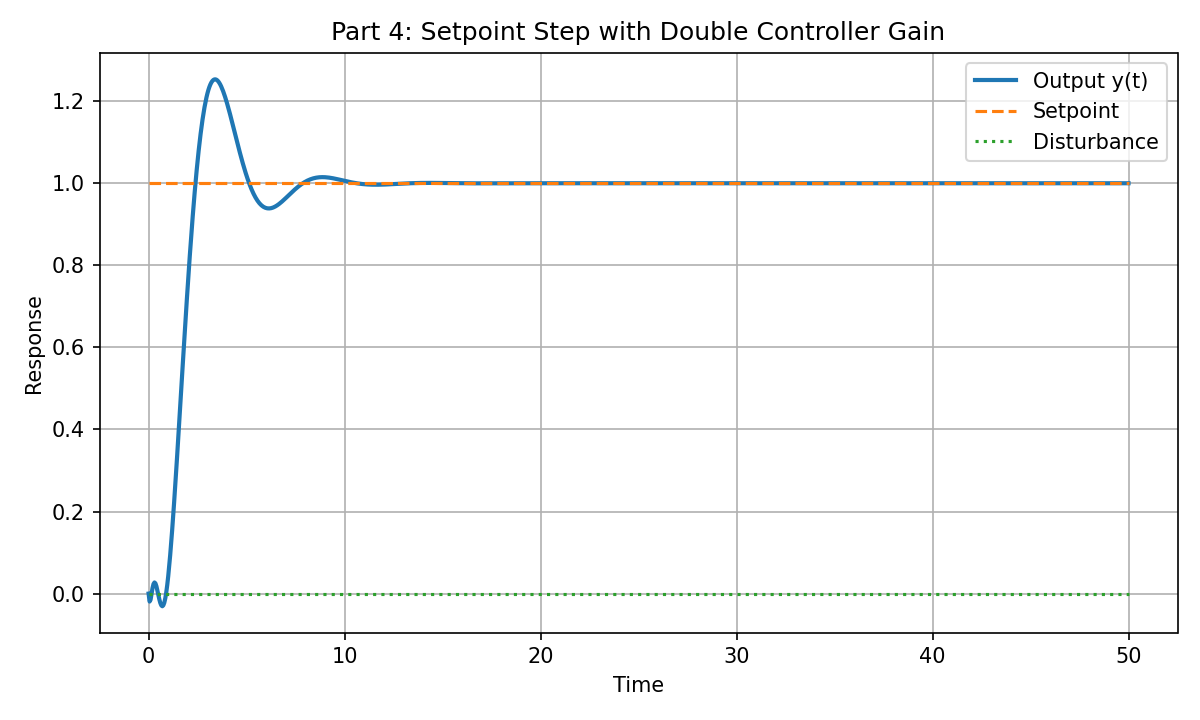
\includegraphics[width=0.95\textwidth]{part4_setpoint_kc_double.png}%
\caption{Closed{-}loop response to a unit step in setpoint with doubled controller gain.}%
\label{fig:fig3}%
\end{figure}

%


\begin{figure}[H]%
\centering%

\includegraphics[width=0.95\textwidth]{part4_disturbance_kc_double.png}%
\caption{Closed{-}loop response to a unit step in disturbance with doubled controller gain.}%
\label{fig:fig4}%
\end{figure}

%
\[%
\text{For the doubled controller gain, the setpoint response is shown in Figure} \ref{fig:fig3}  \text{, and the disturbance response is shown in Figure} \ref{fig:fig4}.%
\]%
The controller gain was then reduced to half of its nominal value and the simulations of Parts 2 and 3 were repeated.%
\par%
\begin{align*}%
K_c^{\text{half}} &= 0.5(1.8750) = 0.9375%
\end{align*}%


\begin{figure}[H]%
\centering%
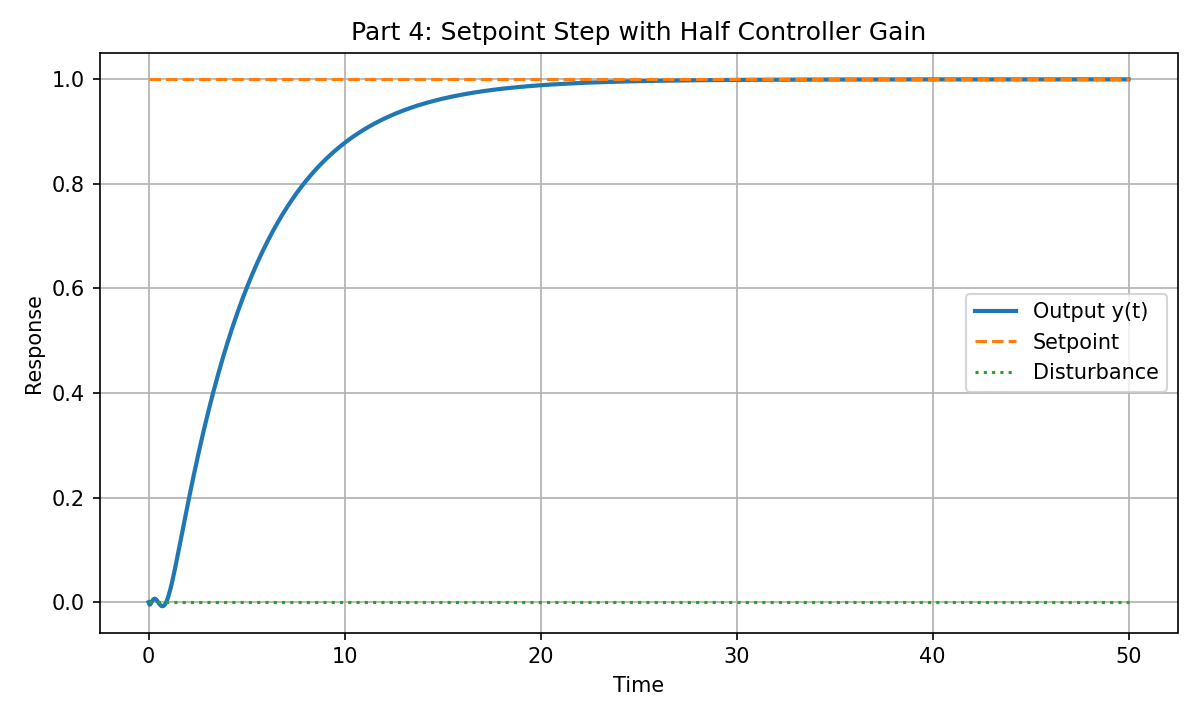
\includegraphics[width=0.95\textwidth]{part4_setpoint_kc_half.png}%
\caption{Closed{-}loop response to a unit step in setpoint with half the nominal controller gain.}%
\label{fig:fig5}%
\end{figure}

%


\begin{figure}[H]%
\centering%

\includegraphics[width=0.95\textwidth]{part4_disturbance_kc_half.png}%
\caption{Closed{-}loop response to a unit step in disturbance with half the nominal controller gain.}%
\label{fig:fig6}%
\end{figure}

%
\[%
\text{For the halved controller gain, the setpoint response is shown in Figure} \ref{fig:fig5} \text{, and the disturbance response is shown in Figure} \ref{fig:fig6}.%
\]%


\begin{figure}[H]%
\centering%
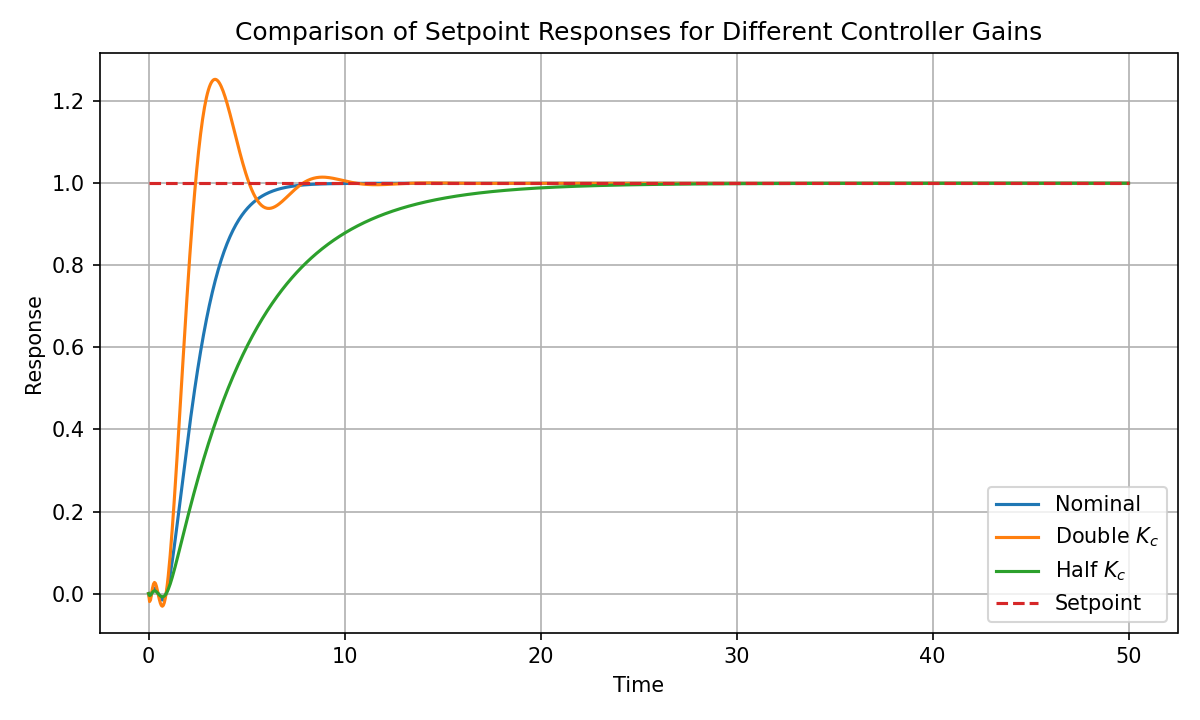
\includegraphics[width=0.95\textwidth]{compare_kc_setpoint.png}%
\caption{Comparison of setpoint responses for nominal, doubled, and halved controller gain.}%
\label{fig:fig7}%
\end{figure}

%


\begin{figure}[H]%
\centering%

\includegraphics[width=0.95\textwidth]{compare_kc_disturbance.png}%
\caption{Comparison of disturbance responses for nominal, doubled, and halved controller gain.}%
\label{fig:fig8}%
\end{figure}

%
\[%
\text{A direct comparison of the gain variations is shown in Figures \ref{fig:fig7} and \ref{fig:fig8}.}%
\]

%
\subsection*{5. Effect of Changing the Integral Time Constant}%
\label{subsec:5.EffectofChangingtheIntegralTimeConstant}%
The controller gain was returned to its nominal value, and the integral time constant was varied above and below its nominal value.%
\par%
\begin{align*}%
K_c &= 1.8750 \\%
\tau_I^{\text{nominal}} &= 5.0000%
\end{align*}%
First, the integral time constant was increased.%
\par%
\begin{align*}%
\tau_I^{\text{large}} &= 2(5.0000) = 10.0000 \\%
I^{\text{large}} &= \frac{1}{10.0000} = 0.1000%
\end{align*}%


\begin{figure}[H]%
\centering%
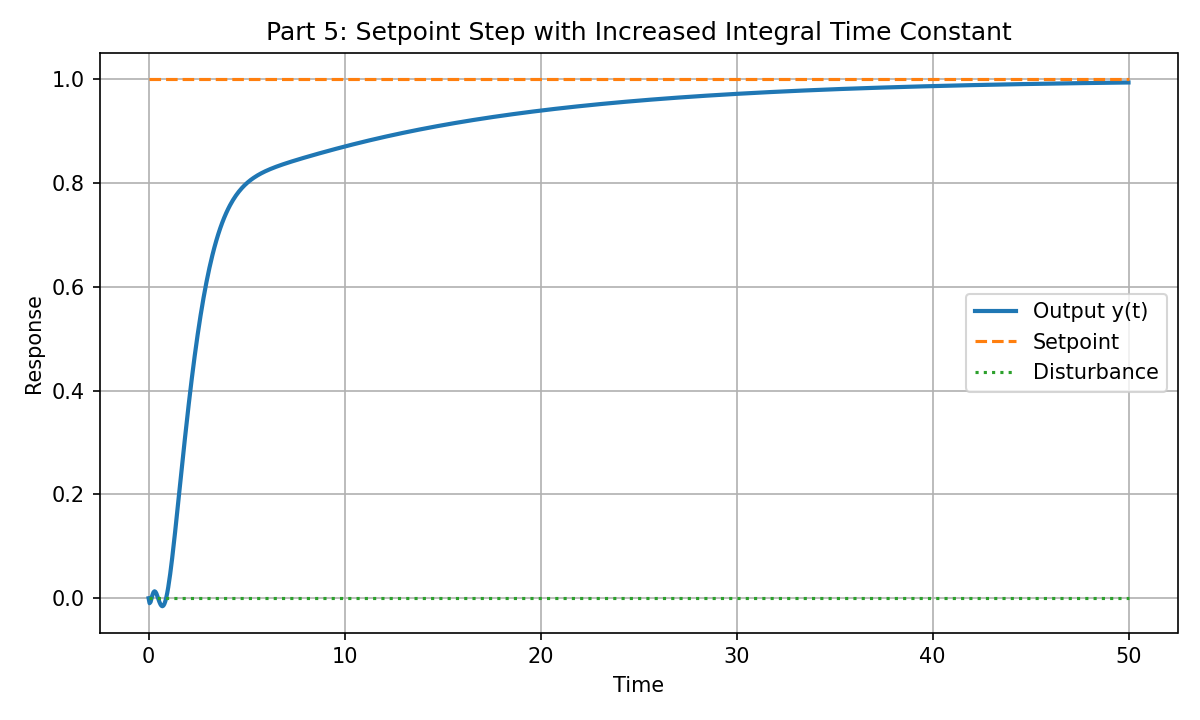
\includegraphics[width=0.95\textwidth]{part5_setpoint_tauI_large.png}%
\caption{Closed{-}loop response to a unit step in setpoint with increased integral time constant.}%
\label{fig:fig9}%
\end{figure}

%


\begin{figure}[H]%
\centering%

\includegraphics[width=0.95\textwidth]{part5_disturbance_tauI_large.png}%
\caption{Closed{-}loop response to a unit step in disturbance with increased integral time constant.}%
\label{fig:fig10}%
\end{figure}

%
\[%
\text{The corresponding setpoint and disturbance responses are shown in Figures \ref{fig:fig9} and \ref{fig:fig10}.%
\]%
Next, the integral time constant was decreased.%
\par%
\begin{align*}%
\tau_I^{\text{small}} &= 0.5(5.0000) = 2.5000 \\%
I^{\text{small}} &= \frac{1}{2.5000} = 0.4000%
\end{align*}%


\begin{figure}[H]%
\centering%

\includegraphics[width=0.95\textwidth]{part5_setpoint_tauI_small.png}%
\caption{Closed{-}loop response to a unit step in setpoint with decreased integral time constant.}%
\label{fig:fig11}%
\end{figure}

%


\begin{figure}[H]%
\centering%
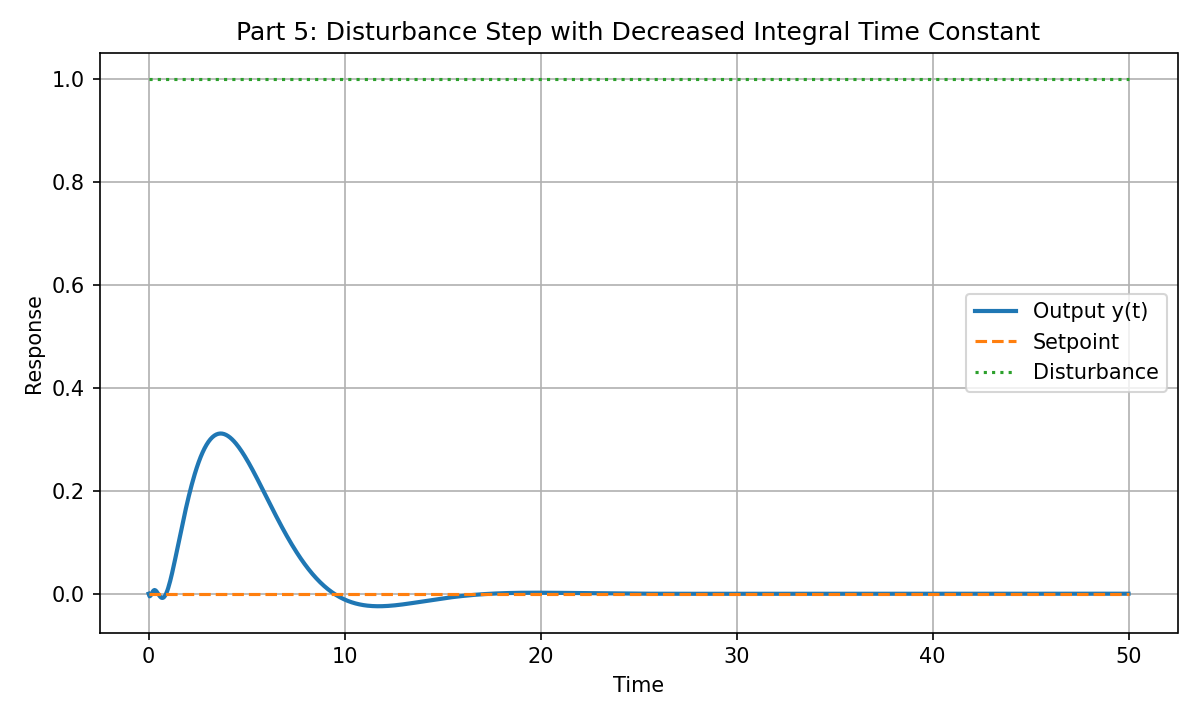
\includegraphics[width=0.95\textwidth]{part5_disturbance_tauI_small.png}%
\caption{Closed{-}loop response to a unit step in disturbance with decreased integral time constant.}%
\label{fig:fig12}%
\end{figure}

%
\[%
\text{The corresponding setpoint and disturbance responses are shown in Figures \ref{fig:fig11} and \ref{fig:fig12}.}%
\]%


\begin{figure}[H]%
\centering%

\includegraphics[width=0.95\textwidth]{compare_tauI_setpoint.png}%
\caption{Comparison of setpoint responses for nominal, increased, and decreased integral time constant.}%
\label{fig:fig13}%
\end{figure}

%


\begin{figure}[H]%
\centering%

\includegraphics[width=0.95\textwidth]{compare_tauI_disturbance.png}%
\caption{Comparison of disturbance responses for nominal, increased, and decreased integral time constant.}%
\label{fig:fig14}%
\end{figure}

%
\[%
\text{A direct comparison of the integral time constant variations is shown in Figures \ref{fig:fig13} and \ref{fig:fig14}.}%
\]

%
\subsection*{6. Comments on the Effects of Changing Controller Parameters}%
\label{subsec:6.CommentsontheEffectsofChangingControllerParameters}%
Increasing the controller gain produced a faster response for both setpoint tracking and disturbance rejection, but the responses became more oscillatory and exhibited greater overshoot.%
\par%
Decreasing the controller gain produced a slower and more sluggish response, but the behavior was generally smoother and less oscillatory.%
\par%
Increasing the integral time constant weakened the integral action because the reset rate decreased. As a result, offset was removed more slowly and the overall response became less aggressive.%
\par%
Decreasing the integral time constant strengthened the integral action because the reset rate increased. This caused the controller to remove offset more quickly, but it also increased the tendency toward oscillation.%
\par%
Overall, the nominal tuning obtained from the lambda rules provided a reasonable balance between response speed and stability.%
\par

%
\subsection*{Final Controller Parameters}%
\label{subsec:FinalControllerParameters}%
\begin{align*}%
K_c &= 1.8750 \\%
\tau_I &= 5.0000 \\%
I &= 0.2000%
\end{align*}

%
\end{document}